\section{Results and Discussion}\label{sec:Results}

% \subsection{Dependence on Number of Fit Points}

% \begin{figure}[p]
%   \centering
%   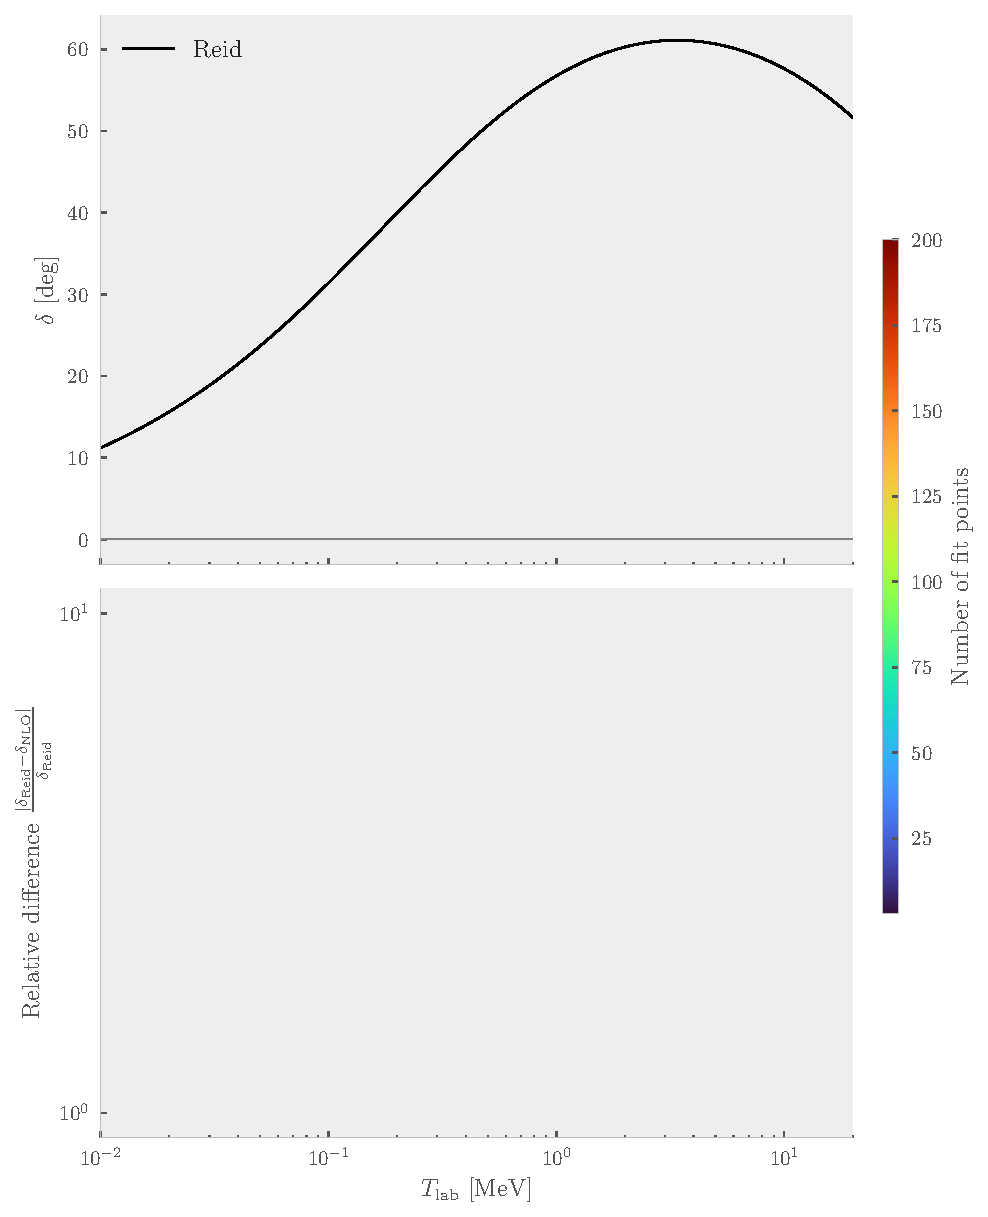
\includegraphics[]{Figures/NLO_points_error.pdf}
%   \caption{\label{fig:points_pointwise} Comparison of Reid and NLO with
%     different number of points used in the minimization. Each curve is fit in
%     the region \([\SI{1e-3}{MeV}, \SI{3}{MeV}]\), resulting in curves shown in the
%     top panel. The pointwise relative error when compared to the Reid potential
%     is shown in the bottom panel. Each curve is colored by the number of points
%     used in the minimization. The minimization gets progressively better as more
%   points are used in the fit.}
% \end{figure}

% \begin{figure}[p]
%   \centering
%   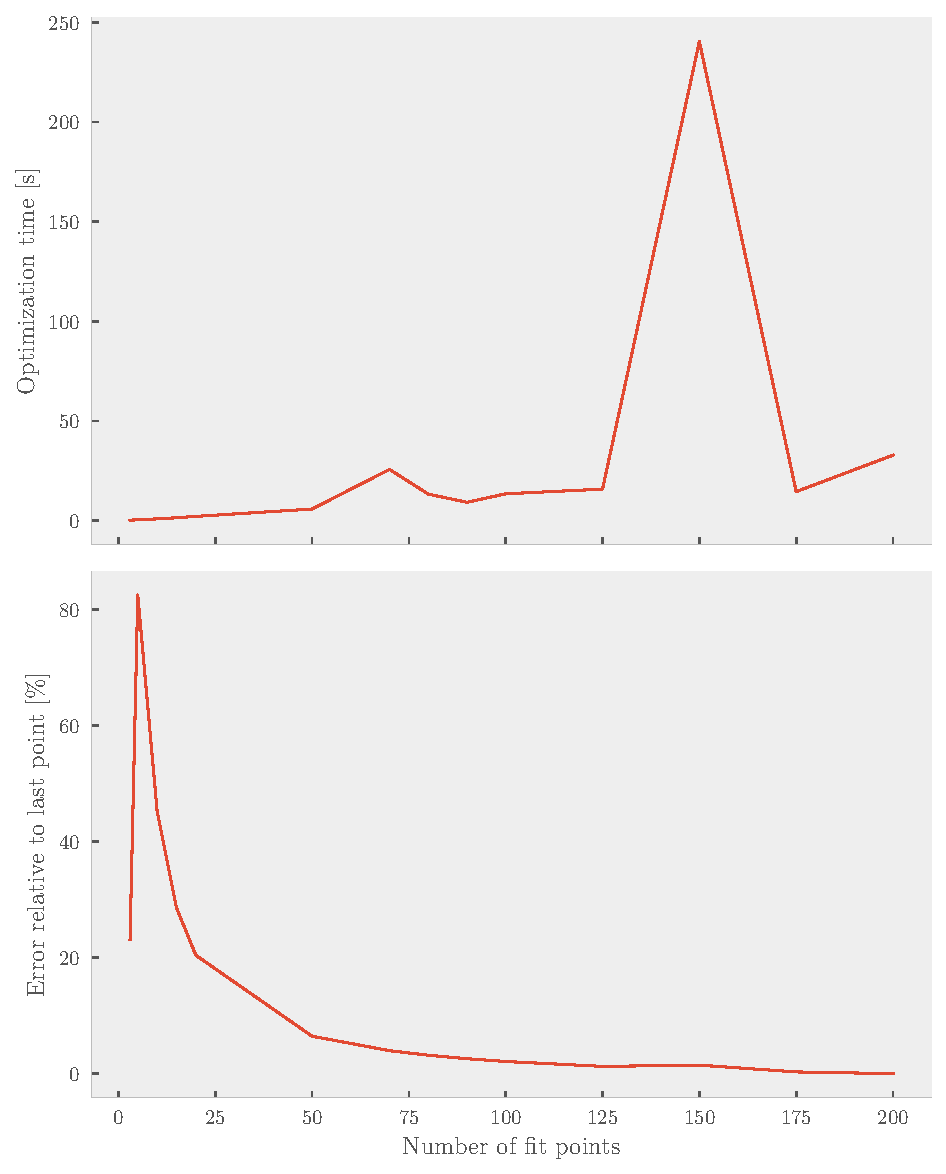
\includegraphics[]{Figures/NLO_dependence_time_error.pdf}
%   \caption{\label{fig:points_time} Illustration of the trade-off between time
%     and accuracy as number of points increases. The time (top panel) increases
%     almost linearly with the number of point, except for the peak \(150\). The
%     error (bottom panel) is calculated as the total relative error when compared
%   to the Reid potential, relative to the last point. Choosing 20 points instead
%   of 200 increases the error by \(20\%\), while \(70\) points yields \(~5\%\)
%   more error.}
% \end{figure}

% \begin{figure}[ht]
%   \centering
%   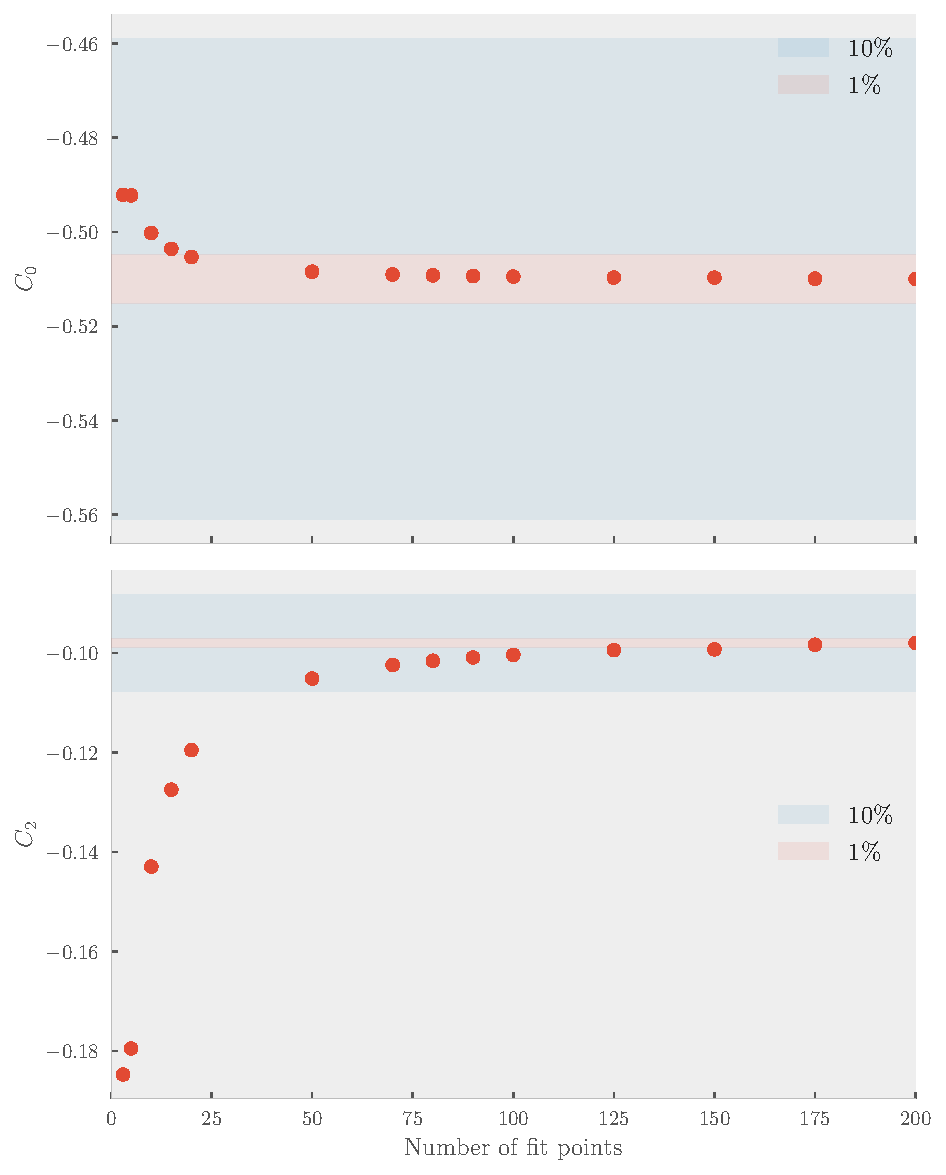
\includegraphics[]{Figures/NLO_coeff_dependence.pdf}
%   \caption{\label{fig:points_coeff} Convergence of the coefficients of NLO as
%   the number of points used in the minimization increases. The shaded bands
%   shows points within \(10\%\) and \(1\%\) of the coefficients value at \(200\)
%   points. At 25 points
%   \(C_{0}\) has already converged to within \(1\%\) of the final value.
%   \(C_{0}\) converges much slower, getting within \(1\%\) of the final value at
%   175 points. }
% \end{figure}

\subsection{Fit at Low Energies}

As recommended by [machleidth], a fit is performed in the range \([10^{-3},
10^{-1}]\) MeV. The resulting phase shift and relative error in the range
\(10^{-3}\) to \(100\) MeV is shown in \cref{fig:lowenergy}. Each order has less
error than the previous in the fit region, converging to the same error as the
energy increases. There is, however, not a massive improvement from NLO to
NNLO, especially when comparing to figure 3 of [machleidt, show here for
reference]. Note also the different shapes of the error curves. Each dip
corresponds to a change in sign of the error, a crossing of the computed phase
shift with the actual phase shift.

The two phase shift results of NNLO illustrate a common problem with our method
of fitting. A completely unconstrained fit, labeled simply ``NLO'', give worse
results than a constrained fit, labeled ``NLO Constrained'', where the
coefficients are forced to be within some hand
picked regions. The reason for this is not clear, but is discussed later. 

The 95\% confidence intervals (CI) of each coefficient is given in


\begin{table}[htb]
  \centering
  \begin{tabular}{l|SSSS}
    \multicolumn{5}{c}{Coefficients}\\
    Potential & \(C_{0}\) & \(C_{2}\) & \(C_{4}\) & \(C_{4}^{\prime}\)\\
    \toprule
    LO& -0.53& \---- & \---- & \---- \\
    NLO& -0.54&0.048& \---- & \---- \\
    NNLO& -0.50&0.054&-0.99& 0.87\\
    NNLO Constrained & -0.52 & 0.37 & -1.18 & -1.85 \\
    \multicolumn{5}{c}{}\\
    \multicolumn{5}{c}{95\% Confidence Interval}\\
    &\(C_{0}\) & \(C_{2}\) & \(C_{4}\) & \(C_{4}^{\prime}\)\\
    \midrule
    LO &2e-6& \---- & \---- & \---- \\
    NLO& 1e-5& 6e-5& \---- & \----\\
    NNLO &3e1& 7e1&6e2&1e3 \\    
    NNLO Constrained &2e1& 4e1 &4e2 & 7e2 \\
  \end{tabular}
  \caption{Coefficients found from fit at \(10^{-3}\) to \(10^{{-1}}\) MeV, as
    well as 95\% confidence intervals of the coefficients. Only the rough
    magnitude is shown for the CI as the numbers change with each execution of
    the fit. [Labels refuse to align. Fix].}
  \label{tab:lowenergy}
\end{table}

\begin{figure}[pt]
  \centering
  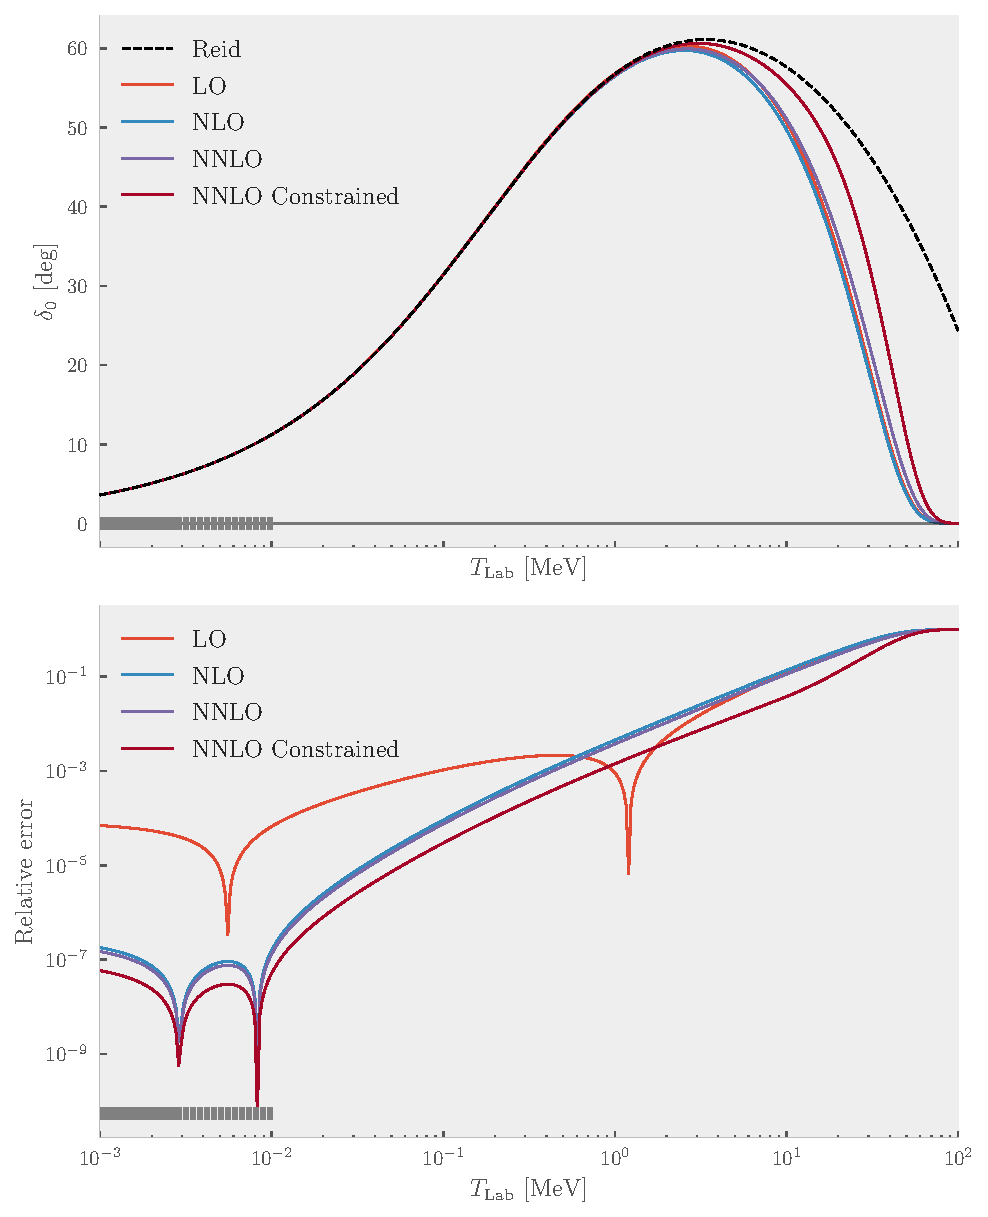
\includegraphics{Figures/lowenergy.pdf}
  \caption{\label{fig:lowenergy} Fit to low energy region with the phase shift
    shown in the top panel and relative error in the lower. The points used in
    the fit is indicated as ticks near the bottom of each plot. LO, NLO and NNLO
  had no limits to their coefficients, while NNLO Constrained was constrained to
 exclude ``unphysical'' phase shifts. The sharp dips are where the curves change
sign.}
\end{figure}

\subsection{Fit at Medium Energies}

To see the effect of including higher energies, another fit was performed from \(10^{-3}\)
to \(1\) MeV. The resulting phase shifts and errors are shown
in~\cref{fig:midenergy}. There is a degradation all around except around \(1\) MeV
when compared to the low energy fit. In particular, NLO is far worse, being
negligibly better than LO. Another noteworthy change is the increasing number of
dips in the NNLO error, suggesting a more complex shape of the phase shift, as
well as NNLO being better able to fit the Reid potential at energies higher than \(1\) MeV.

The coefficients and CI are shown in~\cref{tab:midenergy}. The degradation in LO
and NLO is reflected in the increased uncertainty of the coefficients by some
orders of magnitude. The CIs of NLO are still small when compared to the value of
the coefficient, indicating that the region used in the fit is worse than the
lower energy. On the other hand, the NNLO has markedly smaller CIs, indicating
that the higher energies are necessary for a good fit.

\begin{table}[htb]
  \centering
  \begin{tabular}{l|SSSS}
    \multicolumn{5}{c}{Coefficients}\\
    Potential & \(C_{0}\) & \(C_{2}\) & \(C_{4}\) & \(C_{4}^{\prime}\)\\
    \toprule
    LO& -0.53& \---- & \---- & \---- \\
    NLO& -0.53&0.015& \---- & \---- \\
    NNLO& -0.46&0.44&-2.4& -1.1\\
    \multicolumn{5}{c}{}\\
    \multicolumn{5}{c}{95\% Confidence Interval}\\
              &\(C_{0}\) & \(C_{2}\) & \(C_{4}\) & \(C_{4}^{\prime}\)\\
    \midrule
    LO &1e-5& \---- & \---- & \---- \\
    NLO& 1e-3& 6e-3& \---- & \----\\
    NNLO &4e-1& 6e-1&5e0&1e1 \\    
  \end{tabular}
  \caption{Coefficients found from fit at \(10^{-3}\) to \(1\) MeV, as
    well as 95\% confidence intervals of the coefficients. Only the rough
    magnitude is shown for the CI as the numbers change with each execution of
    the fit. [Labels refuse to align. Fix].}
  \label{tab:midenergy}
\end{table}

\begin{figure}[pt]
  \centering
  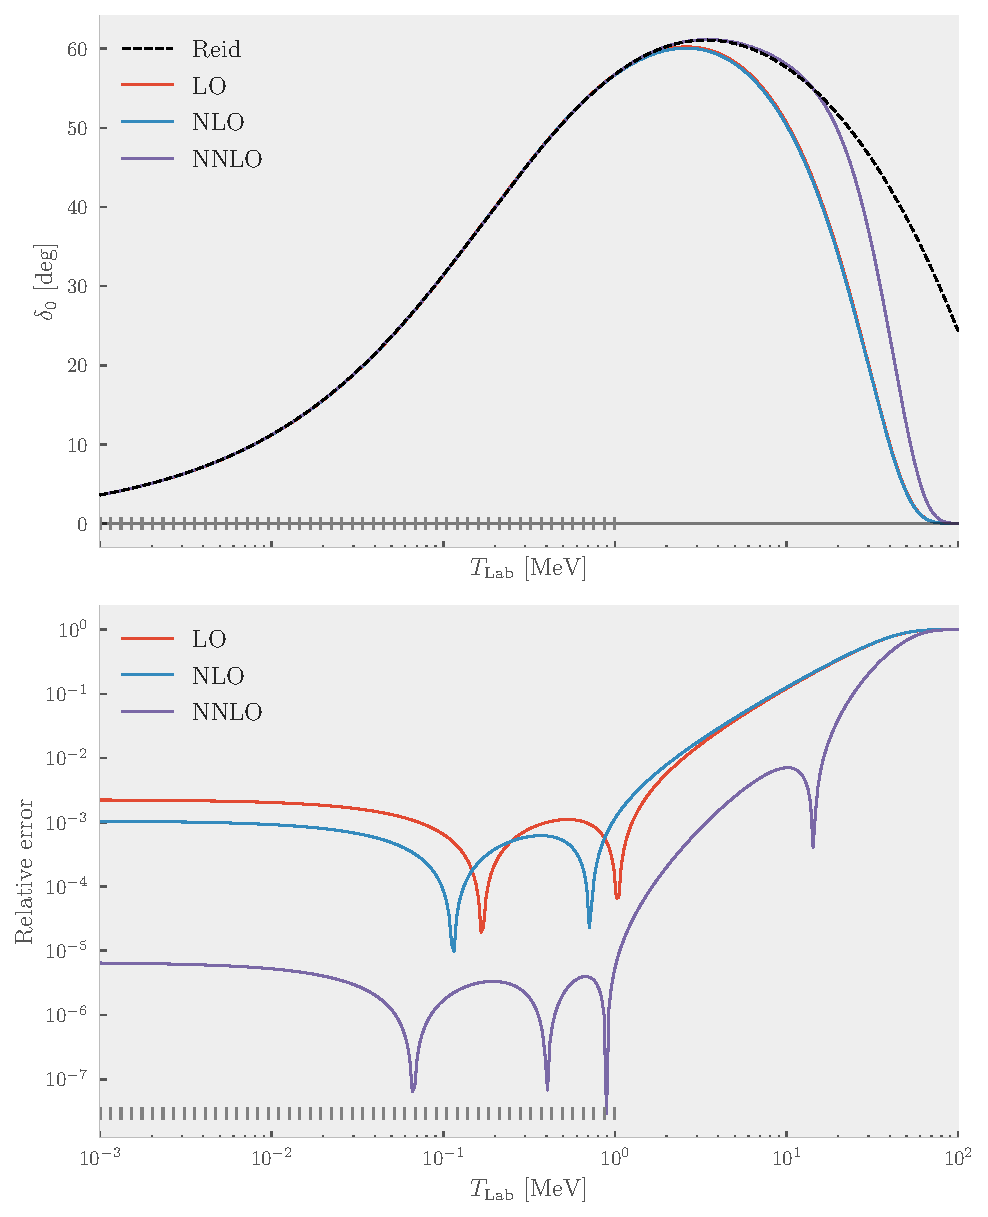
\includegraphics{Figures/midenergy.pdf}
  \caption{\label{fig:midenergy}Fit to the mid energy region with the phase
    shift shown in the top panel and relative error in the lower. The points
    used in the fit are indicated as ticks near the bottom of each plot. No
    constraints were used on the coefficients. When compared to the low energy
    fit, all perform worse in low energy region. NLO does negligibly better than
  LO.}
\end{figure}

\subsection{Fit at High Energies}

Yet another fit was performed at energies \(10^{-3}\) to \(100\) MeV, with
results shown in~\cref{fig:highenergy}, and yet again we see increase in the
relative error. All of the phase shift curves markedly deviate from the phase
shift of the Reid potential. Of the three, NLO has the worst performance, while
the simplest, LO, performs the best.

\cref{tab:highenergy} gives the CIs of the coefficients. The same tale repeats,
with CI becoming increasingly wide. The CIs of the coefficients of NNLO are
utterly useless, spanning six and eight orders of magnitude. It shows that the
least squares method fails at finding any fitting coefficients. Precisely why it
fails is discussed later in~\cref{sec:breakdown-k-matrix}.

\begin{table}[htb]
  \centering
  \begin{tabular}{l|SSSS}
    \multicolumn{5}{c}{Coefficients}\\
    Potential & \(C_{0}\) & \(C_{2}\) & \(C_{4}\) & \(C_{4}^{\prime}\)\\
    \toprule
    LO& -0.53& \---- & \---- & \---- \\
    NLO& -0.40& -0.58& \---- & \---- \\
    NNLO& -0.70&1.3&-3.0& -9.6\\
    \multicolumn{5}{c}{}\\
    \multicolumn{5}{c}{95\% Confidence Interval \((\pm)\)}\\
              &\(C_{0}\) & \(C_{2}\) & \(C_{4}\) & \(C_{4}^{\prime}\)\\
    \midrule
    LO &3e-2& \---- & \---- & \---- \\
    NLO& 1e-1& 6e-1& \---- & \----\\
    NNLO &2e6& 3e6&1e8&1e8 \\    
  \end{tabular}
  \caption{Coefficients found from fit at \(10^{-3}\) to \(100\) MeV, as
    well as 95\% confidence intervals of the coefficients. Only the rough
    magnitude is shown for the CI as the numbers change with each execution of
    the fit. [Labels refuse to align. Fix].}
  \label{tab:highenergy}
\end{table}

\begin{figure}[pt]
  \centering
  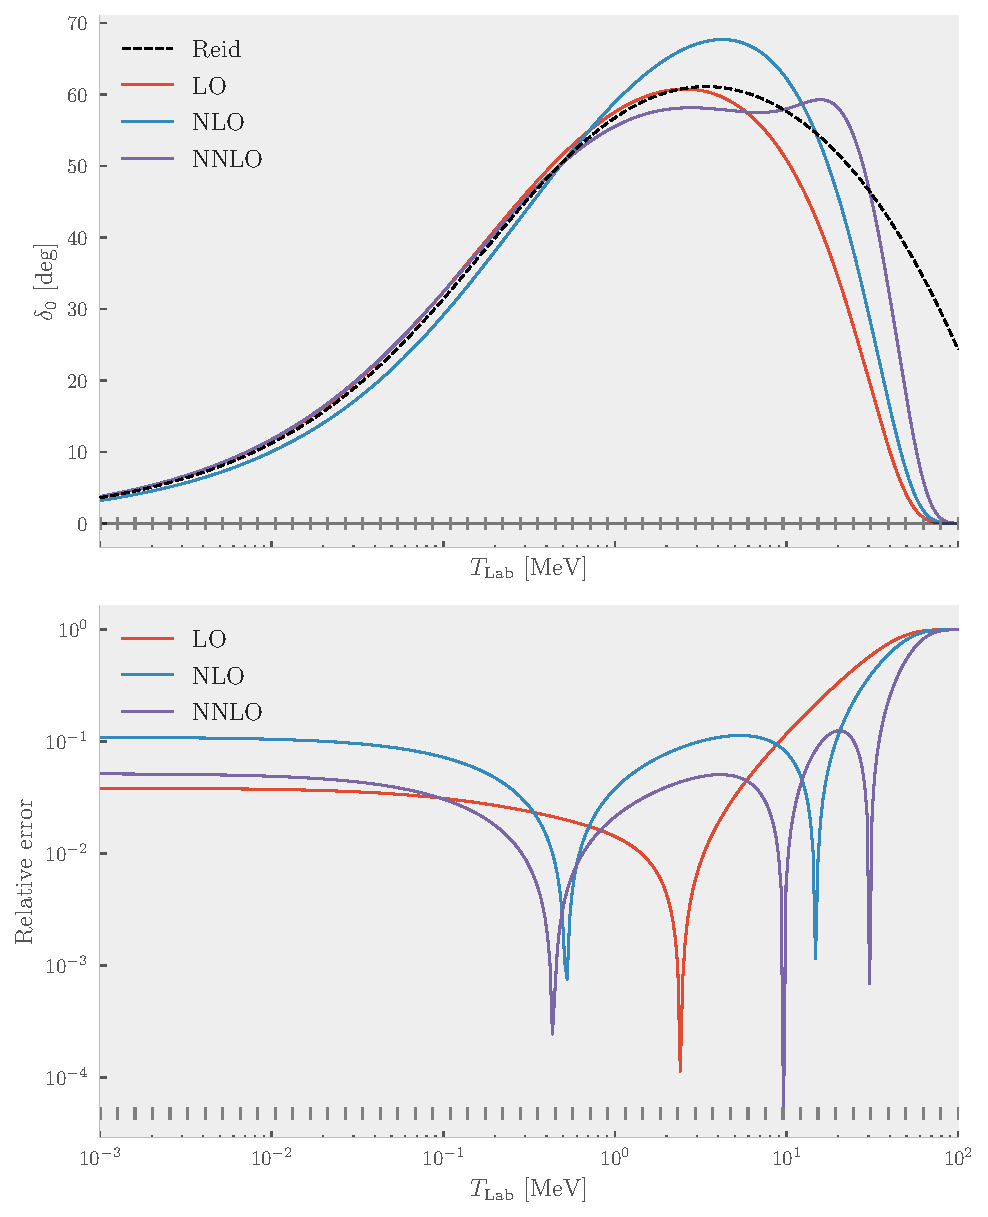
\includegraphics{Figures/highenergy.pdf}
  \caption{\label{fig:highenergy}Fit to the high energy region with the phase
    shift shown in the top panel and relative error in the lower. The points
    used in the fit are indicated as ticks near the bottom of each plot. The
    errors are several order of magnitude greater when compared
    to~\cref{fig:lowenergy} and~\cref{fig:midenergy}}
\end{figure}

\subsection{Dependence on Fit Region}

The previous three sections showed how LO, NLO and NNLO were fitted using
three different \(E_{\mathrm{max}}\) 
Since there seems to be no consensus on what the best fit region is, several
regions were used when fitting the coefficients. LO  is consistently well
behaved, with fast convergence for the minimization procedures and small
dependence on the hyperparameters.

\begin{figure}[pt]
  \centering
  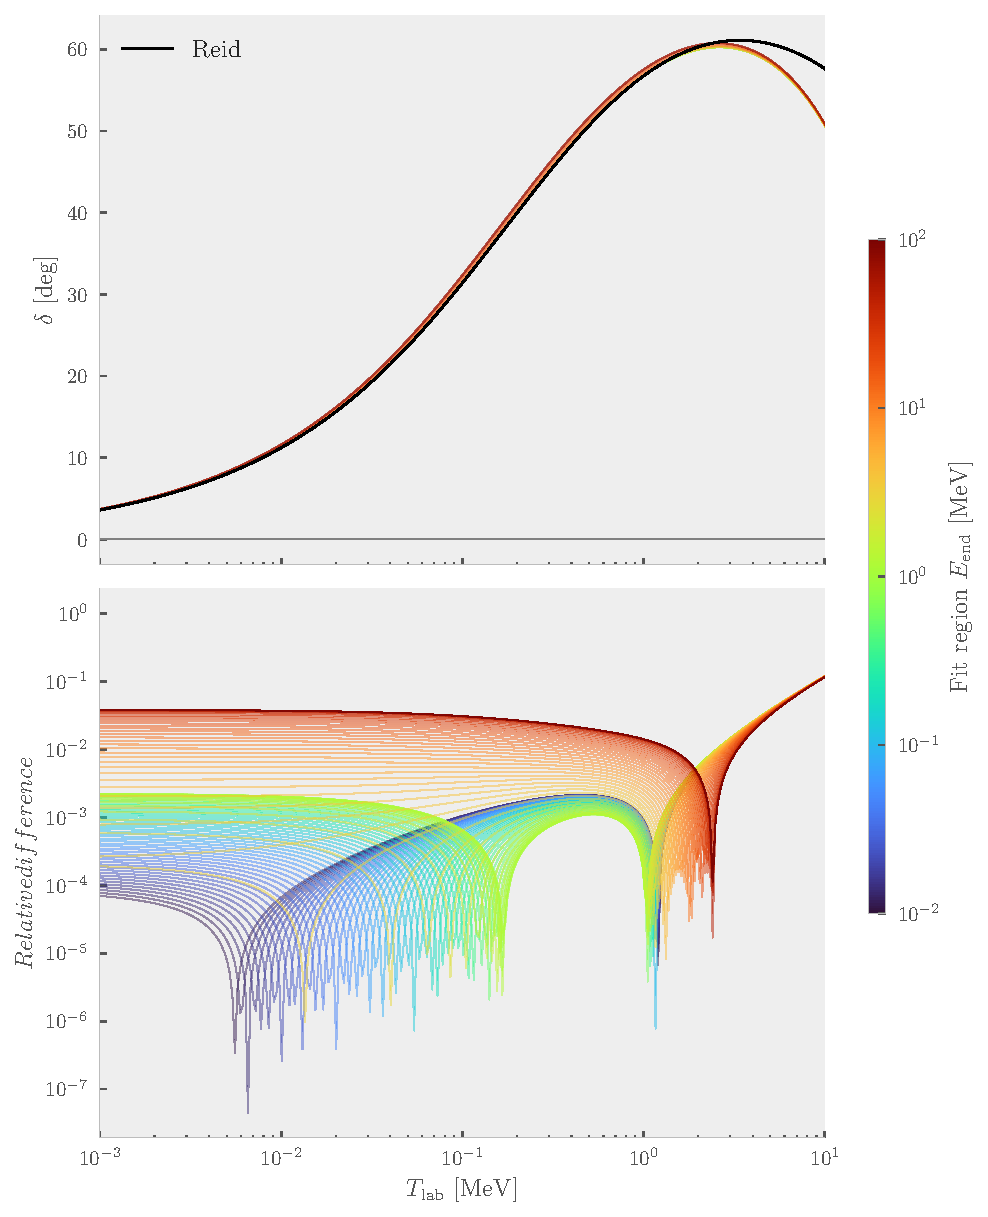
\includegraphics{Figures/LO_region_error.pdf}
  \caption{\label{fig:LO_region_error} }
\end{figure}

\subsection{Breakdown of the K-Matrix method}
\label{sec:breakdown-k-matrix}


% The initial coefficients were \(C_{0} = -0.5, C_{2}=-0.1\),
% \(\Lambda=\SI{0.7}{fm^{-1}}\). There were 50 points within the fit region, and
% the KMatrix method used \(30\) points.

% \begin{figure}[p]
%   \centering
%   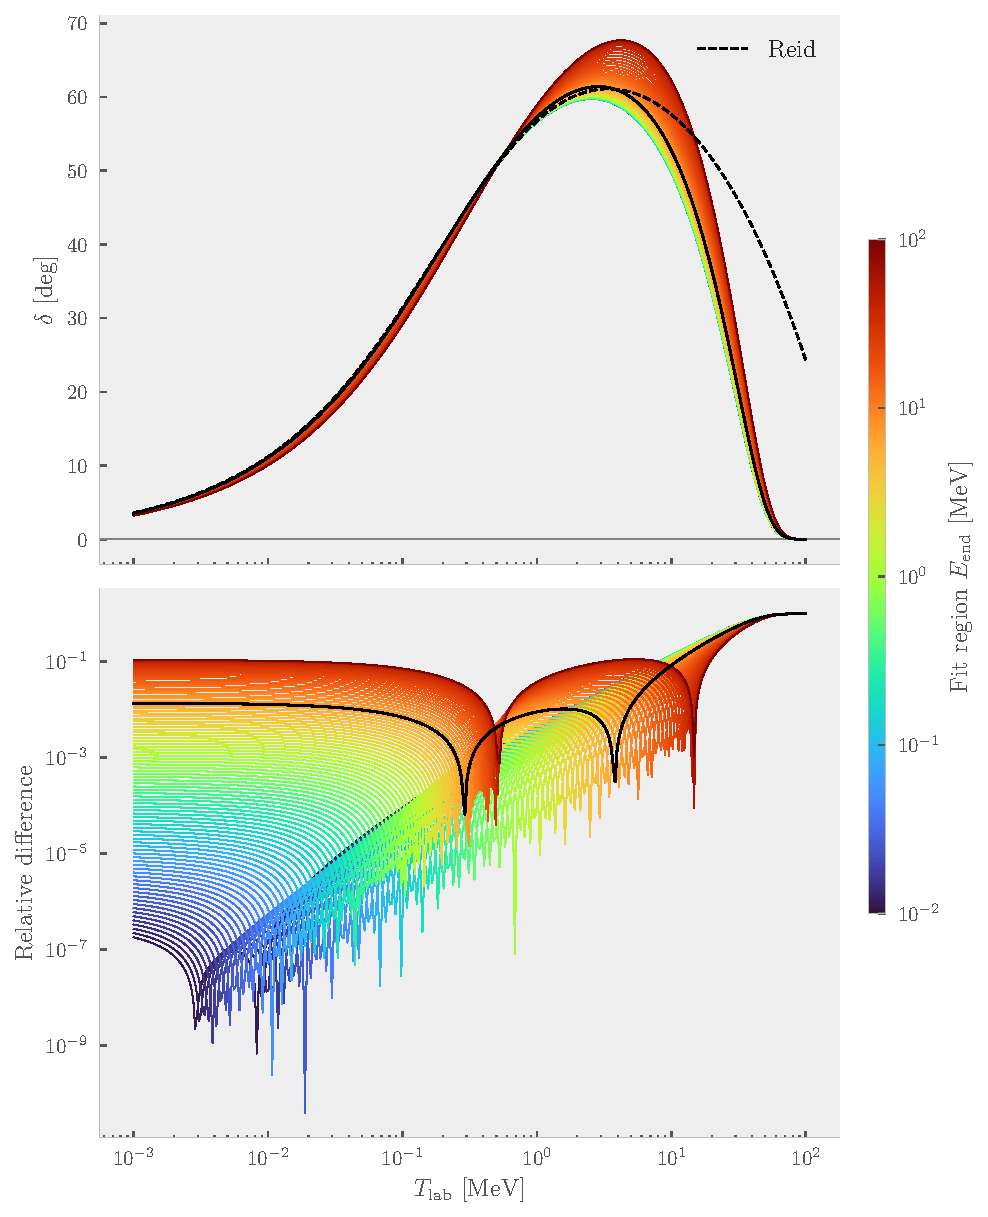
\includegraphics{Figures/NLO_region_error.pdf}
%   \caption{\label{fig:region_pointwise} Comparison of Reid and NLO with
%     different fit regions. Each curve is fit to the region \([10^{-3},
%     E_{\mathrm{end}}]\), with the optimized parameters used to compute the phase
%   shift in \([10^{-3}, 20]\), shown in the upper panel. The relative error
%   compared with Reid is shown in the lower panel. The spikes are artifacts of
%   change of sign, and should be ignored. The curves are colored by the value of
%   \(E_{\mathrm{end}}\) used in the fit. As expected the fit is better at lower
%   values when \(E_{\mathrm{end)}}\) is low, however, large \(E_{\mathrm{end}}\)
%   give drastically worse error. All of the errors converge for \(E > 10\)~MeV.}
% \end{figure}

% \begin{figure}[p]
%   \centering
%   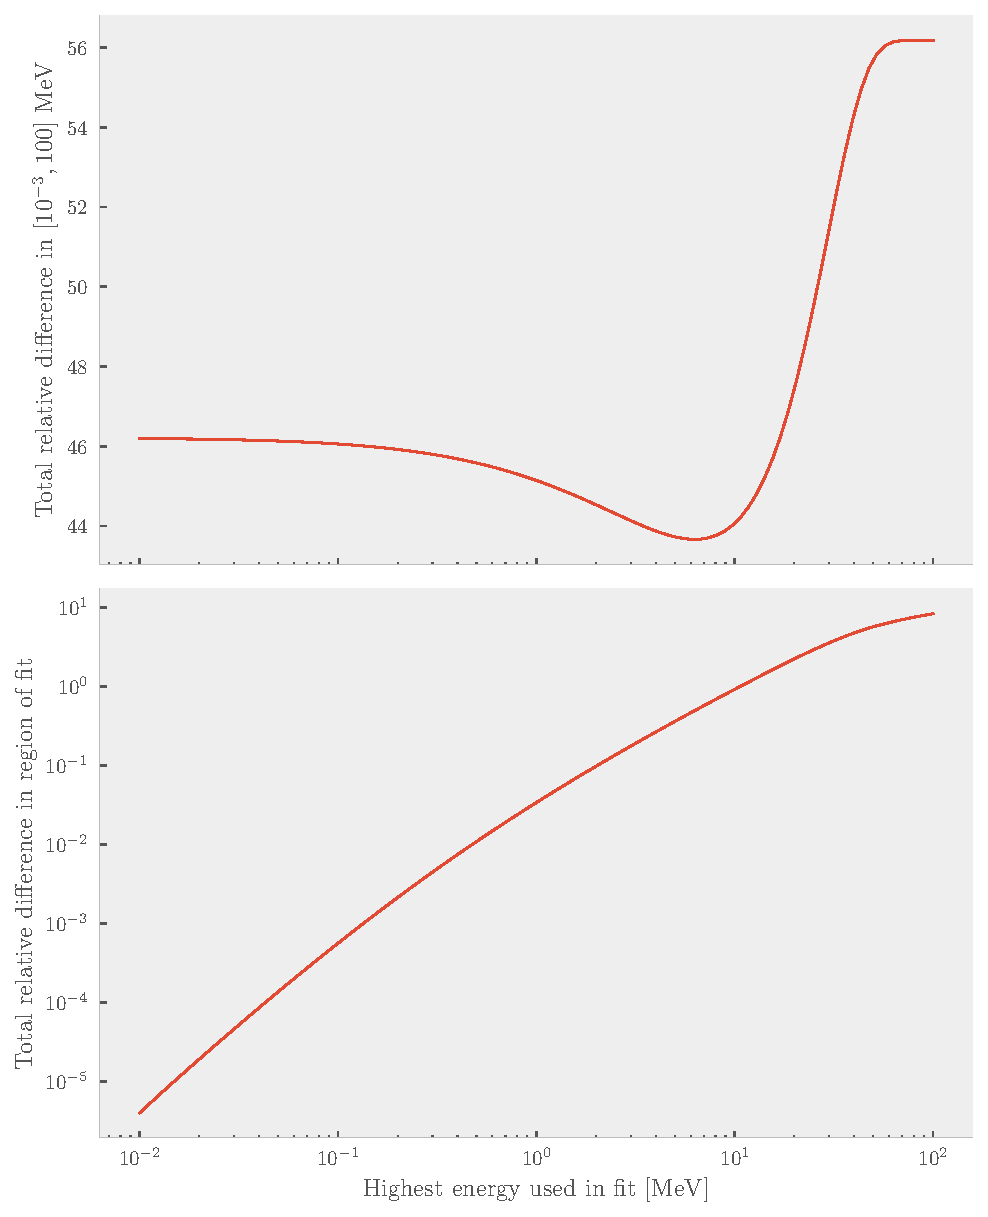
\includegraphics[]{Figures/NLO_dependence_points_error.pdf}
%   \caption{\label{fig:region_total} The time usage (top panel) and total
%     relative error (bottom panel) versus the fit region. The NLO
%     potentials are fit to the region \([\SI{1e-3}{MeV},
%     E_{\mathrm{end}}]\), with the optimized parameters used to compute the phase
%     shift in \([\SI{1e-3}{MeV}, \SI{20}{MeV}]\) and compared to the ``true'' Reid potential. The
%     relative error is summedm giving the curve in the bottom panel. For very low
%     values of \(E_{\mathrm{end}}\) the error is large. The same goes for high
%     values, perhaps unintuitively . The time usage is chaotic for \(E_{\mathrm{end}} <
%     \SI{5}{MeV}\), above which it increases rapidly to several minutes.}
% \end{figure}


% \begin{figure}[p]
%   \centering
%   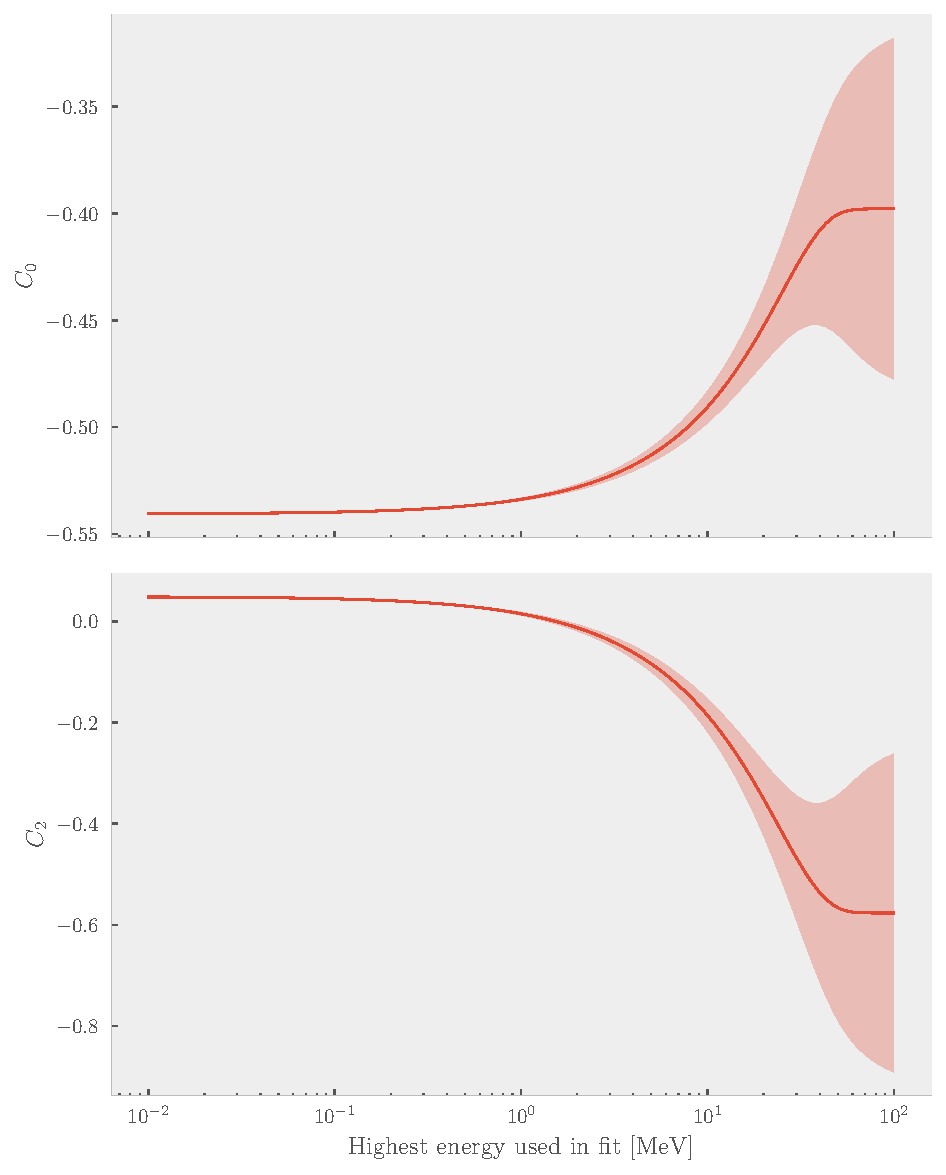
\includegraphics[]{Figures/NLO_coeff_dependence_region.pdf}
%   \caption{\label{fig:region_coeff} The dependence of the coefficients of NLO as
%   a function on \(E_{\mathrm{end}}\). There is no convergence behavior to be
%   seen in the region where the error reaches a minimum. Instead, the behavior is
% purely linear. As NLO is fit to higher energies, \(C_{0}\) increases while
% \(C_{2}\) decreases.}
% \end{figure}

% [stability]
% Coefficients must be initially given to start of the solver, and there might be
% reason for concern about the stability of the solutions. If different
% coefficients were given, would the same solution be achieved? To investigate
% this, the NLO potential was fitted fifty times with random initial coefficients in the
% interval \([-1, 1]\). For coefficients near -1, the matrix in the KMatrix method
% becomes ill conditioned, giving nonsensical results causing the solver to get
% stuck. For other initial coefficients, all solutions converge to the same
% values, agreeing within the tolerance of the optimization method. There is
% therefore no reason to suspect the solver finding local minima.


%%% Local Variables:
%%% mode: latex
%%% TeX-master: "../main"
%%% TeX-engine: xetex
%%% End:
